\chapter{Background}
\label{chp:background}

This chapter exposes the concepts of mutation testing and the problem of useless mutants. 
%In addition, we come up with concepts related to our strategy in special the technologies we instantiate for conduct the experiments. 
%In spite of being succinct, this summary suffices for the purposes of this work. A more precise introduction of mutation testing can be found in \cite{JIA:2011:1, DEMILLO:1978:1, OFFUTT:2001:1, WOODWARD:1993:1}. 
The rest of the chapter is organized as follows: we introduce mutation testing concepts through the process analysis, the importance of design good mutation operators, examples of mutation tools, and the associated cost of the technique. Thereafter we bring the problem of useless mutants up and how we can overcome it. 

\section{Mutation Testing}
Mutation Testing is a fault-based technique: it injects artificial faults into software by creating many copies of the original program, each one containing one (or more) simple fault(s). 
Then it executes the test suite against these copies to check the compliance of the output from that of the original program. 

Mutation Testing has been increasingly studied since it was first proposed in the 1970s \cite{LIPTON:1971:1, DEMILLO:1978:1}. 
Many research papers have appeared on several points of the mutation process seeking to turn Mutation Testing into a practical approach. 

We detail this process in what follows, indicating the automatic and manual parts.

\subsection{The Mutation Analysis Process}
The main aim of mutation testing is adequacy measurement of a test set. 
For this, some steps need to be taken. 
Offutt and Untch \cite{OFFUTT:2001:1} establishes a generic mutation testing process. We illustrate this process in Figure \ref{fig:mutation_process}. 

\begin{figure}[h]
	\centering
	\caption{Mutation Testing Process}
	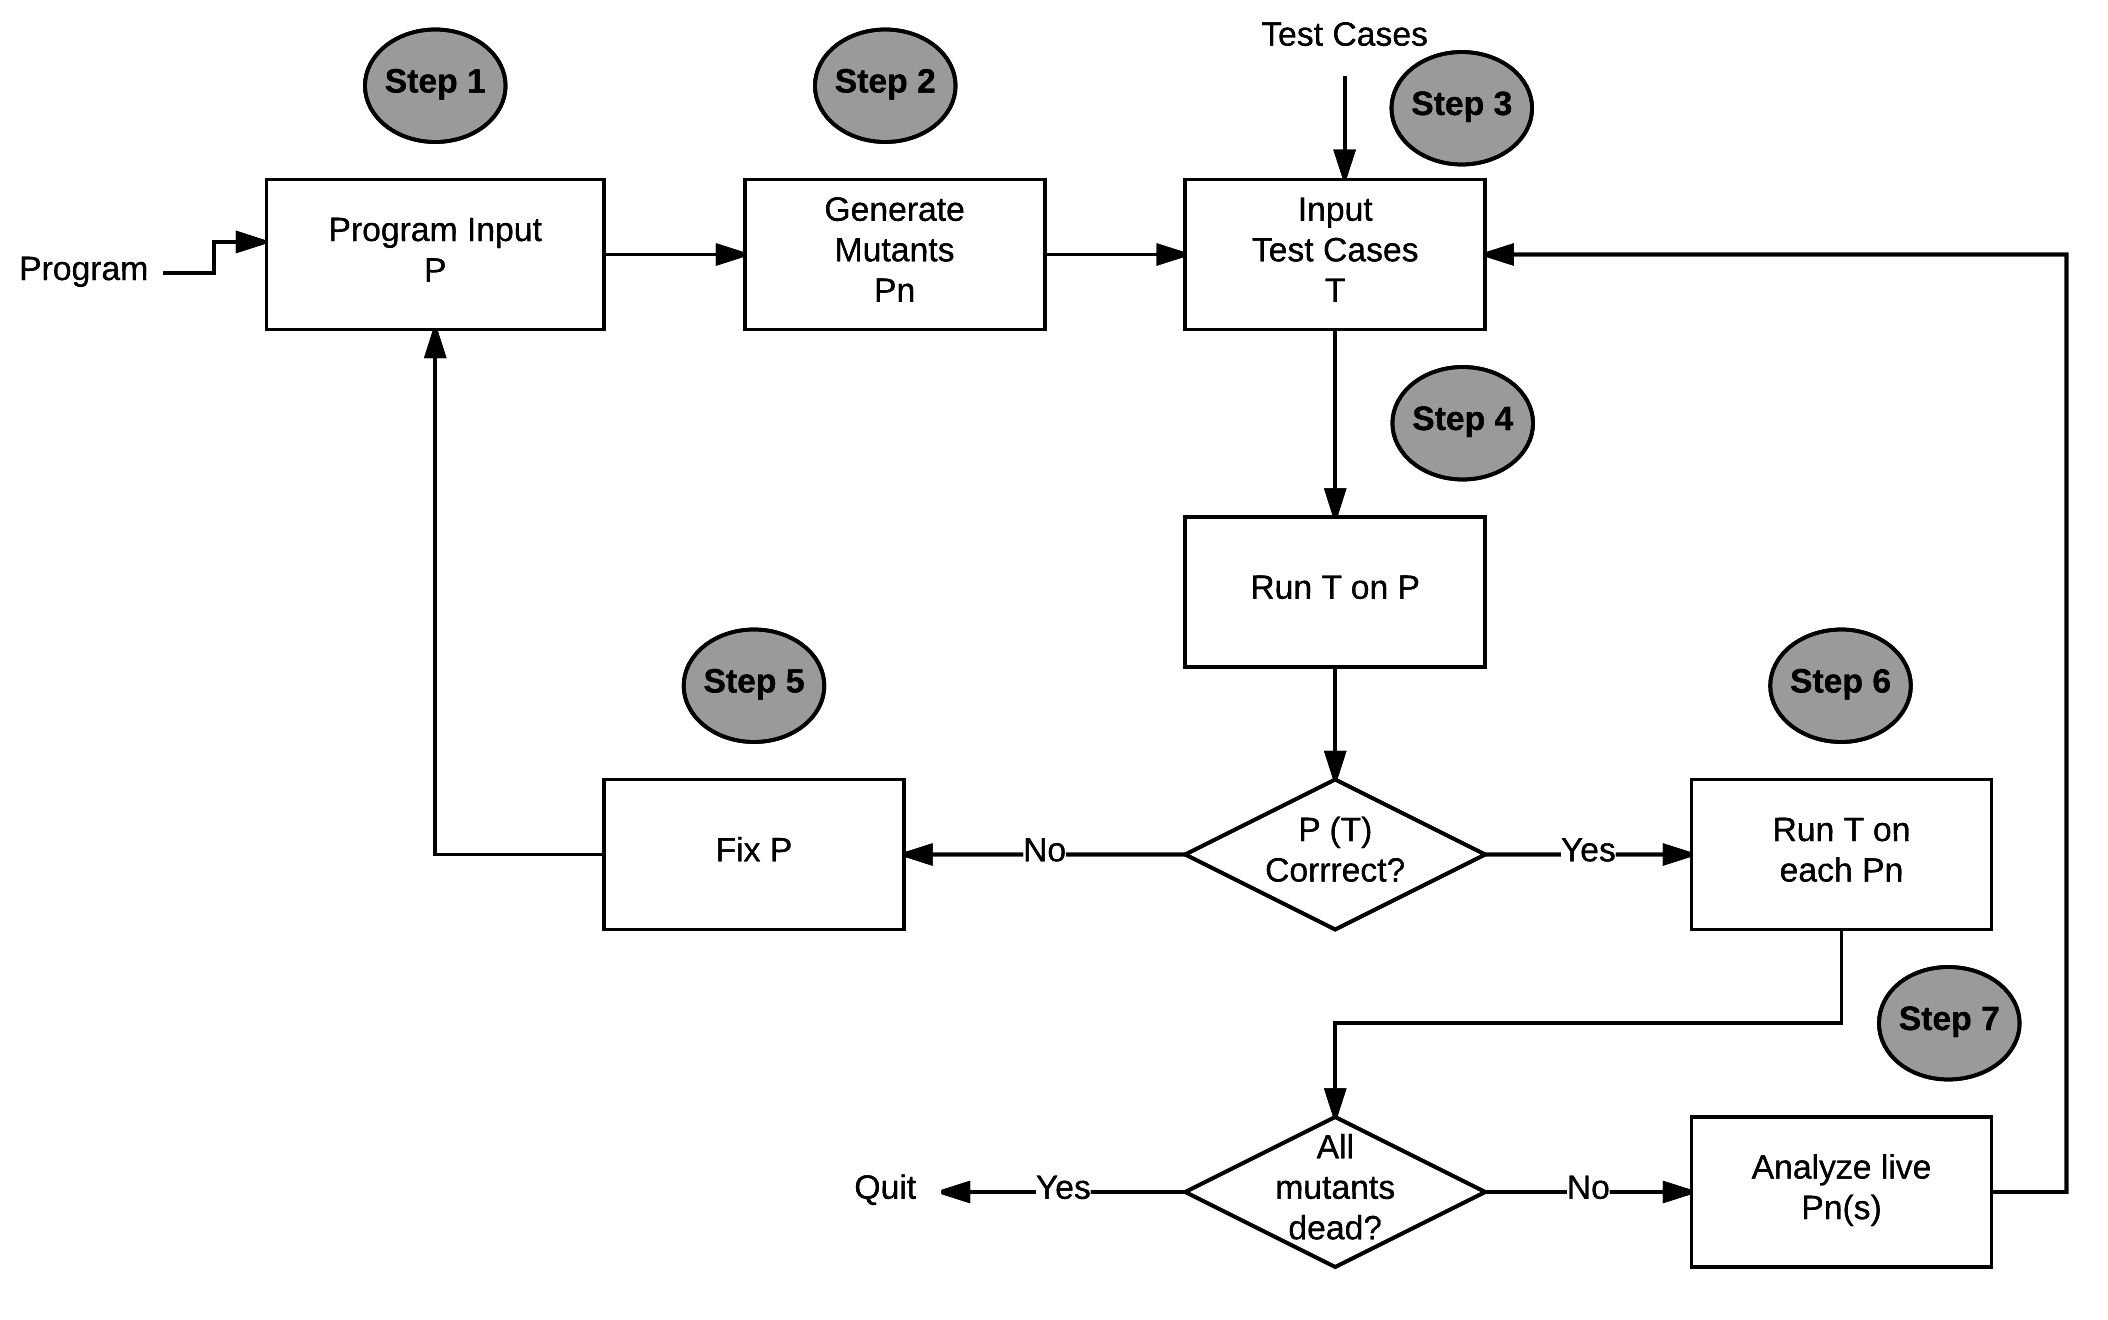
\includegraphics[scale=0.8]{images/mutation-testing-process.png}
	\label{fig:mutation_process}
\end{figure}

Based on an original program input $P$ provided by the developer (Step 1), the mutation testing tool generates a set of faulty programs $Pn$, called \textit{mutants}, by making small syntactic changes from the original program $P$ (Step 2). 
%Figure \todo{...} shows examples of mutations for common statements in imperative languages. 
In the next step, a test set $T$ is supplied to the system (Step 3), and we run $T$ on $P$ (Step 4). 
In case $T$ detects an error in $P$ it is necessary to fix $P$ and start over (Step 5).
But if no error is detected in $P$, the mutation testing tool executes the test set $T$ against each mutant $Pn$ and check its correctness (Step 6). 
If the result of running $Pn$ is different from the result of running $P$ for at least one test case in $T$, then the mutant $Pn$ is said to be ``\textit{killed}'', otherwise it is said to have ``\textit{survived}''.
In case all mutants have been killed so the process ends, but if there is surviving mutants, the developer analyzes these mutants to mark the equivalent mutants (explained in Section \ref{sec:useless_mutants}) or to improve the test suite to kill the mutants that are still alive (Step 7).

Steps 2, 4 and 6 are executed automatically by the majority of the mutation testing tools. 
Steps 1, 3, 5 and 7 need a manual intervention.

The mutation testing tool concludes with an adequacy score to indicate the quality of the test set $T$. The most common adequacy score is the \textit{mutation score}. It is the ratio of the number of killed mutants over the total number of mutants minus the total of equivalents. 

\[ MS=\frac{Mk}{Mt - Me} \]

Where $Mt$ is the total number of produced mutants, $Mk$ is the number of killed mutants and $Me$ is the number of equivalent mutants.
The final value of the mutation score ranges between zero and one, so the closer to one indicates a better result.

When we talk about killing, the way a mutant is killed during the execution process can be classified into three types: \textit{strong}, \textit{weak}, and \textit{firm mutation}. 
%Strong Mutation is often referred to as traditional Mutation Testing \todo{citar 66}. 
% In Strong Mutation, for a given program $P$, a mutant $Pn$ of program $P$ is said to be killed only if mutant $Pn$ gives a different output from the original program $P$.
% In Weak Mutation \todo{citar 115}, instead of checking mutants after the execution of the entire program (or until call the proper output), the mutants need only to be checked immediately after the execution point of the mutant or mutated component.
    % That is, once the mutated component is executed we can check its internal state immediately after the execution of the mutated components and compare with the original program.

In weak mutation~\cite{HOWDEN:1982}, a test kills a mutant if the test execution leads to a difference between the program state of the mutant and the program state of the original version immediately after the execution of the mutated point. 
In contrast, strong mutation~\cite{DEMILLO:1978:1}, often referred to as traditional mutation testing, requires that this difference propagates to an observable output, i.e., an assertion failure or an exception.
Weak mutation is less computationally expensive than strong mutation since we just need to execute the test until the mutated point.
However, given that it is easier to kill weak mutants, then we will sacrifices test effectiveness for improvements in test effort.
This raises the question as to what kind of trade-off can be achieved.
The idea of firm mutation~\cite{WOODWARD:1988:1} is to overcome the disadvantages of both weak and strong mutations by providing a continuum of intermediate possibilities. 
That is, the ``compare state'' of firm mutation lies between the intermediate states after execution (weak mutation) and the final output (strong mutation).
To the best of our knowledge, there is no publicly available firm mutation tool.
In this work, we use the traditional idea of killing a mutant using strong mutation.

In the next section we take a look at the first automated step (Step 2) of a mutation tool. 
The generation of the mutants.

\subsection{Mutants Creation}
Mutants contain faults that are simple syntactic changes based on specific rules known as \textit{mutation operators}. 
Typical mutation operators are designed to modify variables and expressions using replacement, insertion or deletion operators. 
The first objective of a mutation operator is to mimic typical faults that programmers can commit, such as using the wrong operator or omitting a statement.
And the second objective is forcing tests that are usually considered valuable, such as forcing expressions to have the value zero or forcing the execution of all paths in a conditional statement.

The design of mutation operators is crucial to the success of the mutation tool.
The tool must generate as few mutants as possible without losing effectiveness, which means to simulate the maximum number of bugs, but, preferably without incurring in duplicated mutants.
Generate hard-to-kill mutants (also known as stubborn mutants \cite{YAO:2014:1}) help developers to improve their test suite and trivial-to-kill mutants offers no benefits, however, this task is not trivial. 
Besides that, the operators are very dependent on the programming language of choice. For example, the set of operators for Java must be different for the set of operators for Haskell, since the errors that programmers of these languages make tend to be different. 

When a mutant is created by changing one single code location we say it is a \textit{first order mutant}. 
In case the mutant is generated changing more than one place we say it is a \textit{high order mutant} \cite{JIA:2008:1}. 
%\textit{Second order mutants} are the most common \textit{high order mutant}, however 
Tools that implement high order mutants are still scarce \cite{MADEYISKI:2014:1}. 
In this work, we use tools that create first order mutants.
%X and Y \todo{Ref. revisao de mut. equiv.} proposed different algorithms to combine \ac{fom} to generate the second order ones.

\subsection{Mutation Testing Tools}
To make the use of the mutation technique possible, we need tools.
In this work we have selected the following tools to generate the mutants:
\mujava{}~\cite{OFFUTT:2005:1, OFFUT:2006:1}, \major{}~\cite{JUST:2011:1}, and \pit{}~\cite{PIT:2017}.

\mujava{} (Mutation System for Java) \cite{OFFUTT:2005:1, OFFUT:2006:1}, is one of the oldest Java mutation testing tools and has been used in many mutation testing studies. 
The tool manipulates the source code of the program under test and supports two types of mutation operators: class-level and method-level. 
The class-level mutation operators were designed for Java classes and it handles object-oriented specific features such as inheritance, polymorphism, and dynamic binding \cite{MA:2002:1, OFFUT:2006:1}. 
Method-level (traditional) mutants are based on the selective operator set by Offutt et al. \cite{OFFUT:1996:1} and it handles primitive features of the languages.
%Table \todo{montar tabela} presents the operators of the tool, along with a succinct description of the performed changes.
After creating mutants, \mujava{} allows the tester to enter and run tests automatically.
Equivalent mutants must be identified by hand.
In April 2015, \mujava{} has been released as open source under the Apache license.\footnote{\url{https://github.com/jeffoffutt/MUJAVA}}

%Artigo Kintis compara as ferramentas e site
\pit{} \cite{PIT:2017} is a mutation testing framework that targets primarily the industry but has also been used in many research studies.
%Table \todo{Table PIT} describes the corresponding operators. 
%By comparing this table with Table \todo{Tabela MUJAVA}, it can be seen that PIT implements differently specific mutation operators of MUJAVA, for instance, the changes imposed by PIT's Conditionals Boundary operator are a subset of the ones of MUJAVA's Relational Operator Replacement (ROR). 
%Additionally, it employs mutation operators that are not implemented in MUJAVA, e.g. the Void Method Calls and Constructor Calls operators.
\pit{} mutates the bytecode, i.e, it does not compile the code but instead modifies the byte code in memory and \pit{} only requires the location of the source code in order to generate a human readable report.
It employs mutation operators that affect primitive programming language features.
For this work, we extend \pit{} to write all generated mutants in the disk. 
This is important to the equivalent and duplicated analysis. 
\pit{} has been released as open source under the Apache license.\footnote{\url{https://github.com/hcoles/pitest}}

%Artigo Kintis compara as ferramentas e paper sobre a ferramenta
\major{} \cite{JUST:2011:1} is integrated into the Java compiler, in a non-invasive way, and does not require a specific mutation analysis framework. 
The tool manipulates the AST of the program under test. 
The implemented mutation operators are based on a reduced set of operators defined by Offutt et al. \cite{OFFUT:1996:1}, similarly to \mujava{}.
%Table \todo{montar tabela MAJOR} summarizes \major{}'s operators and their imposed changes. 
%As observed by \cite{Kintis:2016}, compared to MUJAVA's operators, it is evident that the two tools share many mutation operators, but implement them differently. 
%Compared to PIT, most operators of MAJOR impose a superset of changes with respect to the corresponding ones of PIT and there are operators of PIT that are completely absent from MAJOR.
\major{} uses mutant schemata \cite{UNTCH:1993:1}. 
That is, to reduce the number of generated versions it produces a \textit{metaprogram} that is derived from the program under study and contains multiple mutations.
Each mutation is guarded by a conditional statement that can be switched on and off at runtime.
To use the mutant for further equivalence analysis, the tool exports each generated mutant to an individual source-code file.
\major{} can be downloaded for free, but does not have its source code released.\footnote{\url{http://mutation-testing.org/}}
%end of the tool explanation

Although they are very mature tools, they do not have embedded solutions to solve some of the inherent cost problems of mutation testing.
%The literature reviews about this theme \cite{JIA:2011:1, MADEYISKI:2014:1} demonstrated a  growing academic interest in mutation testing over the years and its expansion to a vast number of platforms/languages. 
%However, this same interest has not been accompanied by industry, mainly because of the cost barrier. 
In the last years solutions have been proposed to reduce the cost of use mutation testing in real world scenarios. 
We now check some of them.

\subsection{Cost Reduction Techniques}
The barriers that prevent the practical use of mutation testing can be classified into two groups: computational cost and manual labor cost.

The major computational cost of mutation testing arises from the high number of generated mutants and the high computing time to execute each mutant.
Offut and Untch \cite{OFFUTT:2001:1} classify three strategies to solve this problem: \textit{do fewer}, \textit{do faster}, and \textit{do smarter}. 
The ``do fewer'' approaches try to decrease the number of mutants generated without losing effectiveness. 
The ``do faster'' approaches focus on ways of generating and running the mutants as quickly as possible. 
The ``do smarter'' approaches look for clever solutions to generate and run mutants, such as running only the test cases that are necessary for each mutant or distribute the computational expense over several machines. 
%Table \todo{fazer tabela com solucoes} brings the last solutions to computational cost reduction.
For a more detailed list of advances in this field, please refer to \cite{JIA:2011:1, OFFUTT:2001:1}.

% \scriptsize
% \begin{table}
% 	\caption{...}
% 	\centering
% 	\begin{tabular}{|c|c|c|}
% 		\hline
% 		\textbf{Approach} & \textbf{Description} & \textbf{References} \\
% 		\hline
% 		X & Y & Z \\
% 		\hline
% 	\end{tabular}
% 	\label{tab:solutions_computational_cost}
% \end{table}
% \normalsize

In a recent work, Papadakis et al. \cite{PAPADAKIS:2015:1} highlight the problem of \textit{duplicated mutants}. 
That is, two mutants that are equivalent to each other, even if they are not equivalent to the original program from which they are constructed; either one or the other of these two mutually equivalent mutants can be discarded, saving some effort. 
This work tackles this problem and it is better discussed in the next section.

The other side of the cost problem comes from the manual labor cost, i.e. the amount of human effort involved to do some tasks. 
The first one is also known as the \textit{Human Oracle Problem} and claim that the developer needs to know the program's output to assert a testing criterion. 
This problem is inherent to all forms of testing. 
Advances in automatic test case generation can support this laborious task. 
The second one is the Equivalent Mutant Problem. 
Although syntactically different from the original program, the mutant can be semantically equal, which implies that their behavior does not change to any input data, thus the developer needs to check whether a survived mutant is merely hard to kill (one more test case is necessary) or equivalent (no test can kill it, so any attempt will be futile).

This work focuses on the problems of equivalent and duplicated mutants, which \cite{PAPADAKIS:2015:1} names as \textit{useless mutants}. 
The next section explains in more detail the problem of useless mutants.

\section{Useless Mutants}
\label{sec:useless_mutants}
We use the term \textit{useless} to represent equivalent and duplicated mutants. 
These mutants do not incorporate anything to the mutation testing process \cite{PAPADAKIS:2015:1}. 

Equivalent mutants, as explained, occur when the mutant maintains the same behavior as the original program. 
It is a well-known impediment to the practical adoption of mutation testing. 
Budd and Angluin \cite{BUDD:1982:1} have already proven that this is an undecidable problem in its general form. 
Thus, no complete automated solution exists. 
To worsen the situation, manually detecting equivalent mutants is an error-prone and time-consuming task. 
Acree~\cite{ACREE:1980:1} showed that 20\% of the studied mutants were erroneously classified, i.e., a killable mutant classified by mistake as equivalent or vice versa. 
Shuler et al.~\cite{SHULER:2013:1} showed that developers take, on average, 15 minutes to manually classify a mutant as equivalent or nonequivalent.
This problem becomes quite relevant when empirical studies report that between 10\% and 40\% of all the generated mutants are equivalent \cite{OFFUTT:1994:1, OFFUT:1997:1}.
So solutions, even partial, can greatly help reduce this cost.
%Even though it is an undecidable problem, partial semi-automated solutions have been proposed to diminish its adverse effects. 
%The work of Madeyiski et al.~\cite{MADEYISKI:2014:1} surveyed those solutions \todo{and identified 17 relevant techniques (in 22 articles).}

%...and classified in three categories of techniques to solve this problem: \textit{Detecting}, \textit{Suggesting}, and \textit{Avoiding}. 
%The Table \todo{...} shows those solutions.
%\todo{Continuar...}.

Duplicated mutants are a more recent problem \cite{PAPADAKIS:2015:1, KINTIS:2017:1}. 
That is, if the mutant $P1$ is duplicated to the mutant $P2$, all the tests that kill $P1$ \textit{are exactly the same} that kill $P2$.
Although it does not involve a manual effort as equivalent mutants, duplicated mutants take a worthless computational cost, given that the test set needs to execute against two or more mutants that have the same behavior.
Papadakis et al.~\cite{PAPADAKIS:2015:1} was able to detect 21\% of the mutants as duplicated, however this number may be even higher, since the technique proposed by Papadakis does not detect all cases.
Besides the cost, duplicated mutants make the mutation score imprecise as reported by Kutz et al. \cite{KURTZ:2016:1}. 
For example: Consider a set of 10 nonequivalent mutants $M$ and a set of 10 tests $T$. 
If we execute $T$ against $M$ and it kills 7 mutants, the mutation score is 0.7. 
If 10 more mutants are added to $M$, but all of them are duplicated with a some previous mutant in the set.
That is, there are 20 nonequivalent mutants and 17 are killed, thus the mutation score is now 0.85.
This shows that without any improvement in the test suite the value of the mutation score has changed.
This example and the high number of duplicated mutants that can be generated highlight the importance of having solutions to reduce this problem.

Our work focuses on avoiding useless mutants before they are generated.
In Chapter \ref{sec:strategy} we come up with a strategy to support mutation tool developers to derive rules to avoid useless mutants. 
We show some of these rules in Chapter~\ref{sec:rules} and evaluate them in Chapter~\ref{sec:implementing}.

% \section{Research Status}
% We have included a section on the next steps at the end of all the chapters that follow.
% Here we list what we intend to do about the Background chapter.
% In the Concluding Remarks chapter, we present a schedule for each task.

% \begin{enumerate}
%     \item We plan to extend this chapter by including more details and examples of each concept we use throughout this work.
%     \item We might include examples of common transformations for imperative languages, in special for Java constructs.
%     \item Moreover, we intend to include a list of all mutation operators from the tools we use throughout this work.
%     \item We could also include a table summarizing the main solutions that address the problem of equivalent and duplicated mutants.
%     \item Finally, we plan to extend the Section \ref{sec:useless_mutants} with the redundant mutants that are a more general form of duplicated mutant. 
% \end{enumerate}








%\section{Automated Testing Generation}
%\todo{...}

%\section{Alloy}
%\todo{...}




